%!TEX TS-program = xelatex
%!TEX encoding = UTF-8 Unicode
\documentclass[12pt, xcolor = dvipsnames]{beamer}
\usepackage{style/kcchang-beamer}
\setmainfont[Mapping = tex-text]{Minion Web Pro}
\setsansfont[Mapping = tex-text]{Myriad Web Pro}
\setmonofont[Scale = MatchLowercase]{Operator Mono Book}
\setCJKmainfont[Scale = 0.9, BoldFont = Hiragino Mincho ProN W6]{Hiragino Mincho ProN W3}
\setCJKsansfont[Scale = 0.9, BoldFont = Hiragino Sans W6]{Hiragino Sans W4}
\setCJKmonofont[Scale = 0.9, BoldFont = Yuanti TC Regular]{Hiragino Maru Gothic ProN W4}

\title{Elements of Statistical Learning\\ Chapter 2\\ Overview of Supervised Learning}
\titlegraphic{}
\subtitle{}
\author{Keng-Chi Chang}
%\institute{National Taiwan University}
\date{\today}

\begin{document}
\fontsize{12}{14pt}\selectfont

\maketitle

\begin{frame}
\frametitle{Topics}
\begin{itemize}
  \item Statistical Decision Theory (2.4)
  \item Special Cases: Linear Regression vs. k-Nearest Neighbors (2.3)
  \item Bias-Variance Decomposition (2.9)
  \item Curse of Dimensionality (2.5)
  \item Classes of Restricted Estimators (2.6--2.8)
\end{itemize}
\end{frame}


\begin{frame}
\frametitle{Other References}
\begin{itemize}
  \item \href{http://www-bcf.usc.edu/~gareth/ISL/}{Chapters 2 and 3 of {\it An Introduction to Statistical Learning}}
  \item \href{http://www.stat.cmu.edu/~ryantibs/statml/review/modelbasics.pdf}{Ryan Tibshirani's Lecture Note}
\end{itemize}
\end{frame}


\begin{frame}
\frametitle{Goal: Predict Y from X}
\begin{itemize}
  \item Let $(X,Y)\sim$ iid $P(X,Y)$
  \item Come up with function $f$ to predict $X$ from $Y$
  \item (Squared Error) Loss $L(Y, f(X))=(Y-f(X))^2$
  \item Expected loss $E[(Y-f(X))^2]$ is minimized at $f(x)=E[Y|X=x]$
  \begin{itemize}
    \item Shown by subtracting and adding $E[Y|X]$
  \end{itemize}
  \item $f(x)=E[Y|X=x]$ is called the true regression function
\end{itemize}
\end{frame}


\begin{frame}
\frametitle{Use Data to Estimate $f$}
\begin{itemize}
  \item Now we have (training) data 
  \[D_n=\{(x_1,y_1),\cdots,(x_n,y_n)\,|\,x_i\in\mathbb{R}^p\}\sim \mbox{ iid } P(X,Y)\]
  \item Write $X=(x_1^{T},\cdots,x_n^{T})^{T}$, $Y=(y_1,\cdots,y_n)^{T}$
  \item Use $D_n$ to construct $\hat{f}$ that mimics $f$
  \item That is, we want to find $\hat{f}$ with smaller $E[(Y-\hat{f}(X))^2]$
  \item Notice: $\hat{f}$ depends on data $X$, hence random
\end{itemize}
\end{frame}


\begin{frame}
\frametitle{Use Data to Estimate $f$}
\begin{itemize}
  \item What we can observe is training error
  \[{1\over n}\sum_{i=1}^n{(y_i-\hat{f}(x_i))^2}\]
  \item This is a sample analog of prediction error {\it conditional on the (training) data}
  \[E[(Y-\hat{f}(X))^2\,|\,D_n]\]
  \item Any function $\hat{f}$ passes through $D_n$ can be a minimizing solution
  \item Furthermore, what we really want to know is the {\it unconditional} prediction error that considers data outside $D_n$
  \[E[(Y-\hat{f}(X))^2]=E[E[(Y-\hat{f}(X))^2\,|\,D_n]]\]
\end{itemize}
\end{frame}


\begin{frame}
\frametitle{Linear Regression}
\begin{itemize}
  \item If we believe the relationship between $X$ and $Y$ is close to linear, can make this functional form assumption on $f$ and assume 
  \[f(X)=E[Y|X]\approx X\hat{\beta}=\hat{f}(X)\]
  \item This reduces model complexity (by assuming functional form)
  \item We only need to estimate a finite number of parameters $\beta$
  \item This is a parametric approach to model $f(X)$
\end{itemize}
\end{frame}


\begin{frame}
\begin{center}
  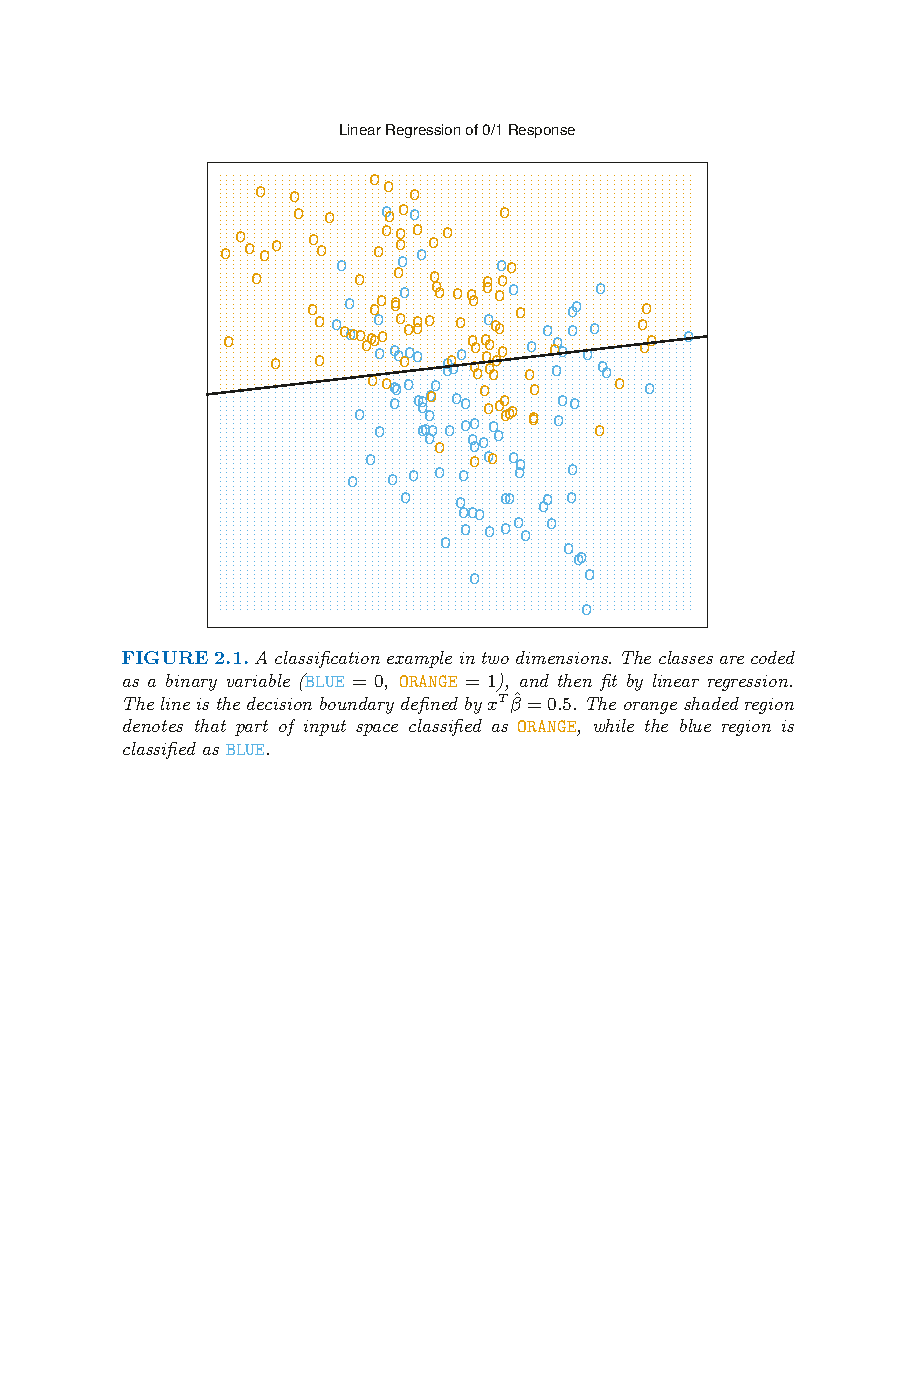
\includegraphics[width=.8\linewidth]{ESL-2-1.pdf}
\end{center}
\end{frame}


\begin{frame}
\frametitle{k-Nearest Neighbors}
\begin{itemize}
  \item One may not want to make functional form assumptions of $f$
  \item One idea: A sample analog of $f(x)=E[Y|X=x]$ can be
  \[\hat{f}(x)={1\over k}\sum_{x_i\in N_k(x)}y_i\]
  where $N_k$ is the set contains all $k$ nearest neighbors of $x$
  \item This is a more flexible class of function
  \item But also comes with costs, since this is similar to estimating infinite dimensions of parameters
  \item This is a non-parametric approach to model $f(X)$
\end{itemize}
\end{frame}


\begin{frame}
\begin{center}
  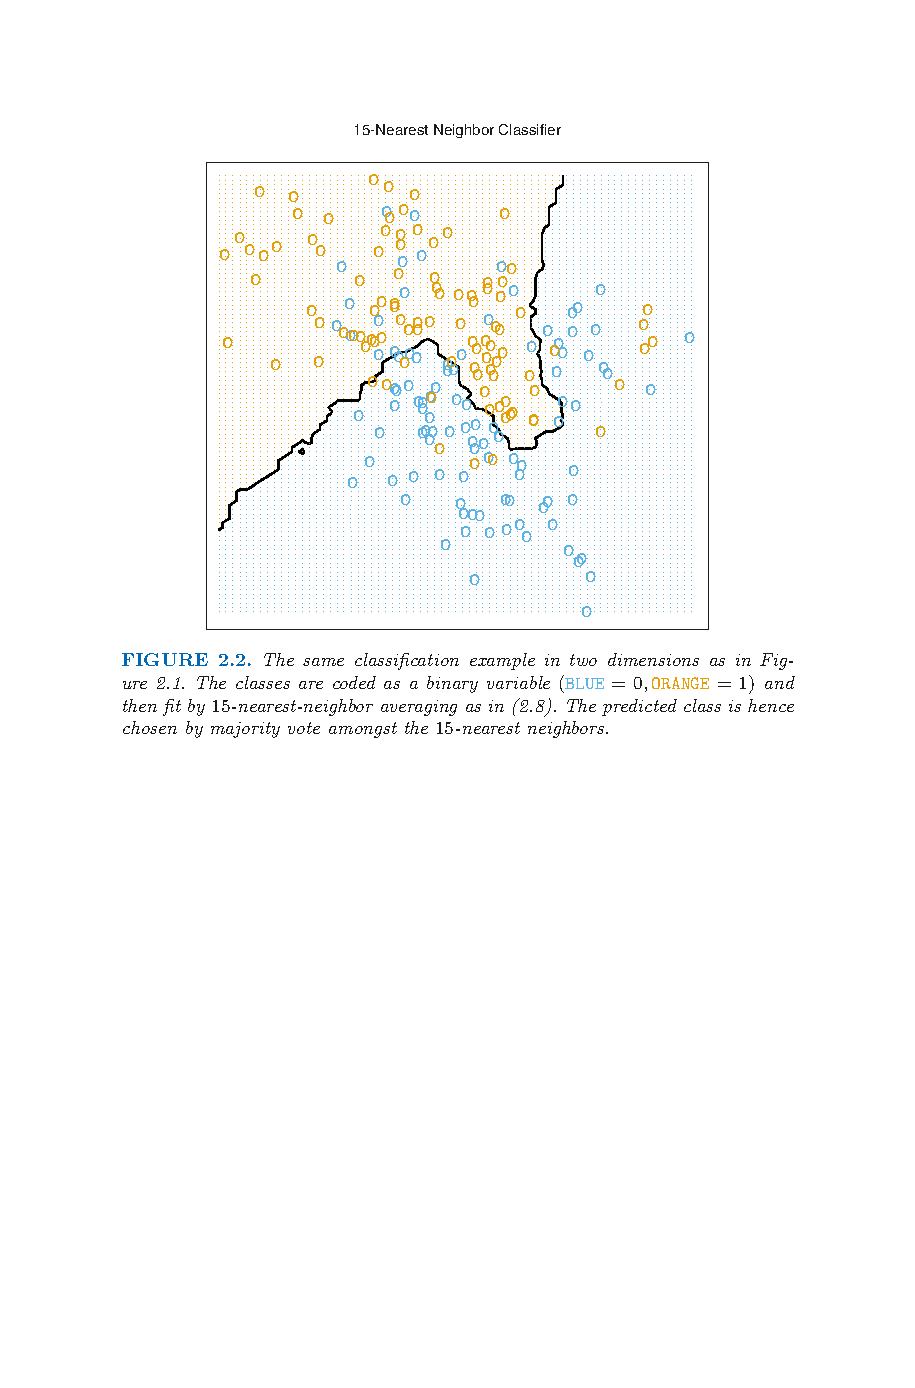
\includegraphics[width=.8\linewidth]{ESL-2-2.pdf}
\end{center}
\end{frame}


\begin{frame}
\begin{center}
  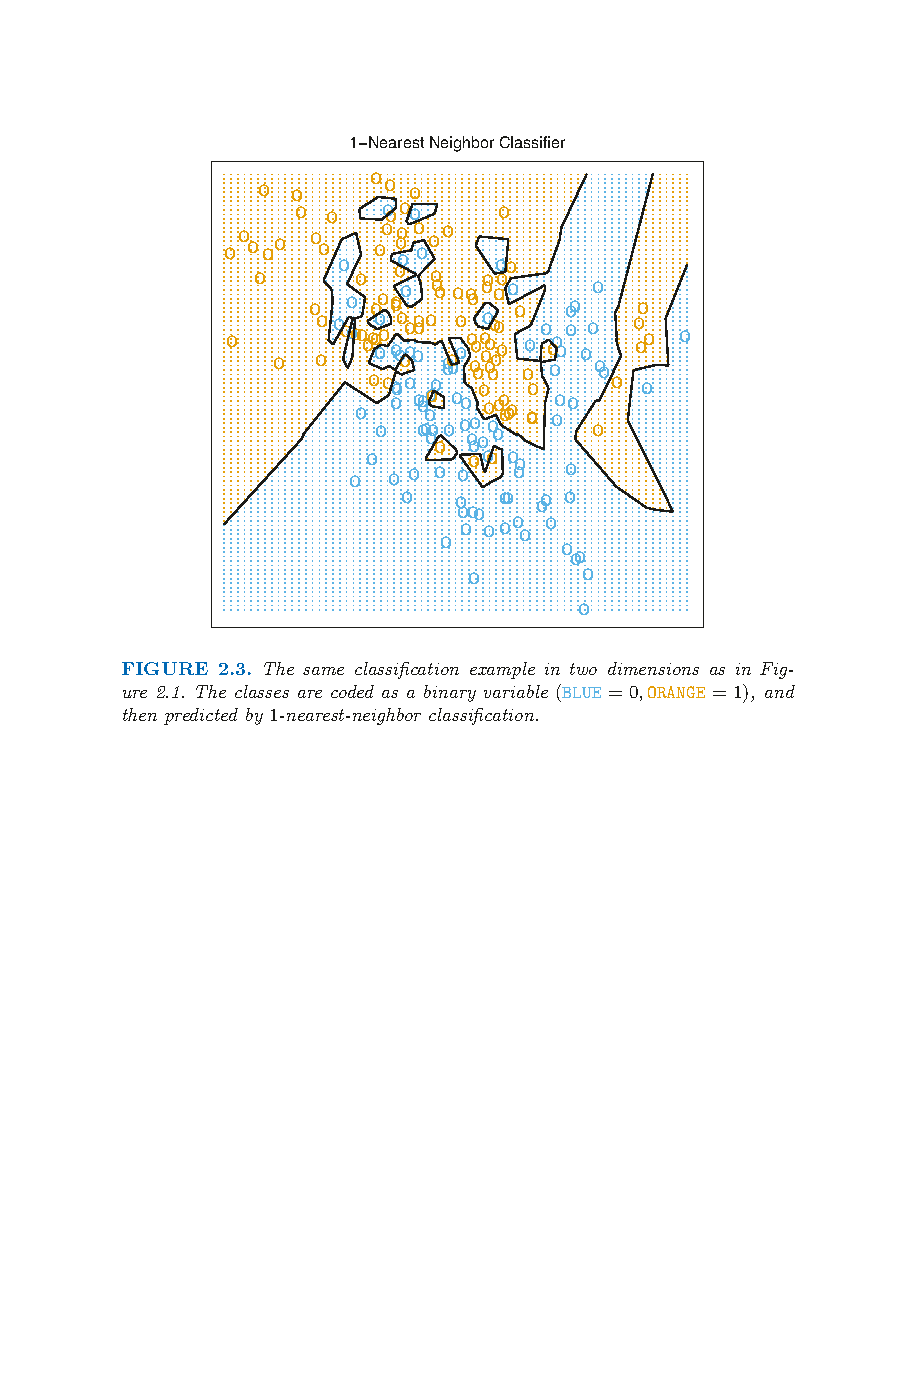
\includegraphics[width=.8\linewidth]{ESL-2-3.pdf}
\end{center}
\end{frame}


\begin{frame}
\frametitle{Irreducible and Mean Squared Errors}
\begin{itemize}
  \item Suppose $Y=f(X)+e$ where $e\sim(0,\sigma^2)$ and $e \perp X$
  \item Conditional on $X=x$, subtracting and adding $f(x)$ from the prediction error, we can write
  \[E[(Y-\hat{f}(X))^2\,|\,X=x]=E[(Y-f(x))^2]-E[(f(x)-\hat{f}(x))^2]\]
  since $E[e]=0$ and $e \perp X$ by construction
  \item $E[(Y-f(x))^2]=\sigma^2$ is irreducible, even if $\hat{f}=f$
  \item $E[(f(x)-\hat{f}(x))^2]=\mbox{MSE}(\hat{f}(x))$ is the mean squared error of the function estimator $\hat{f}(x)$
\end{itemize}
\end{frame}


\begin{frame}
\frametitle{Bias-Variance Decomposition}
\begin{itemize}
  \item Further decompose MSE by subtracting and adding $E[\hat{f}(x)]$
  \[\begin{split}
  E[(f(x)-\hat{f}(x))^2]
  &=E[(f(x)-E[\hat{f}(x)])^2]+E[(E[\hat{f}(x)]-\hat{f}(x))^2]\\
  &=(f(x)-E[\hat{f}(x)])^2+E[(\hat{f}(x)-E[\hat{f}(x)])^2] \\
  &=\mathrm{Bias}^2(\hat{f}(x)) + \mathrm{Var}(\hat{f}(x))
  \end{split}\]
  where the first equality is due to $E[E[\hat{f}(x)]-\hat{f}(x)]=0$
  \item The unconditional prediction error is thus
  \[\begin{split}E[(Y-\hat{f}(X))^2]
  &=E_X[E[(Y-\hat{f}(X))^2|X]] \\
  &=\sigma^2+E_X[\mathrm{Bias}^2(\hat{f}(X))]+E_X[\mathrm{Var}(\hat{f}(X))]
  \end{split}\]
\end{itemize}
\end{frame}


\begin{frame}
\begin{center}
  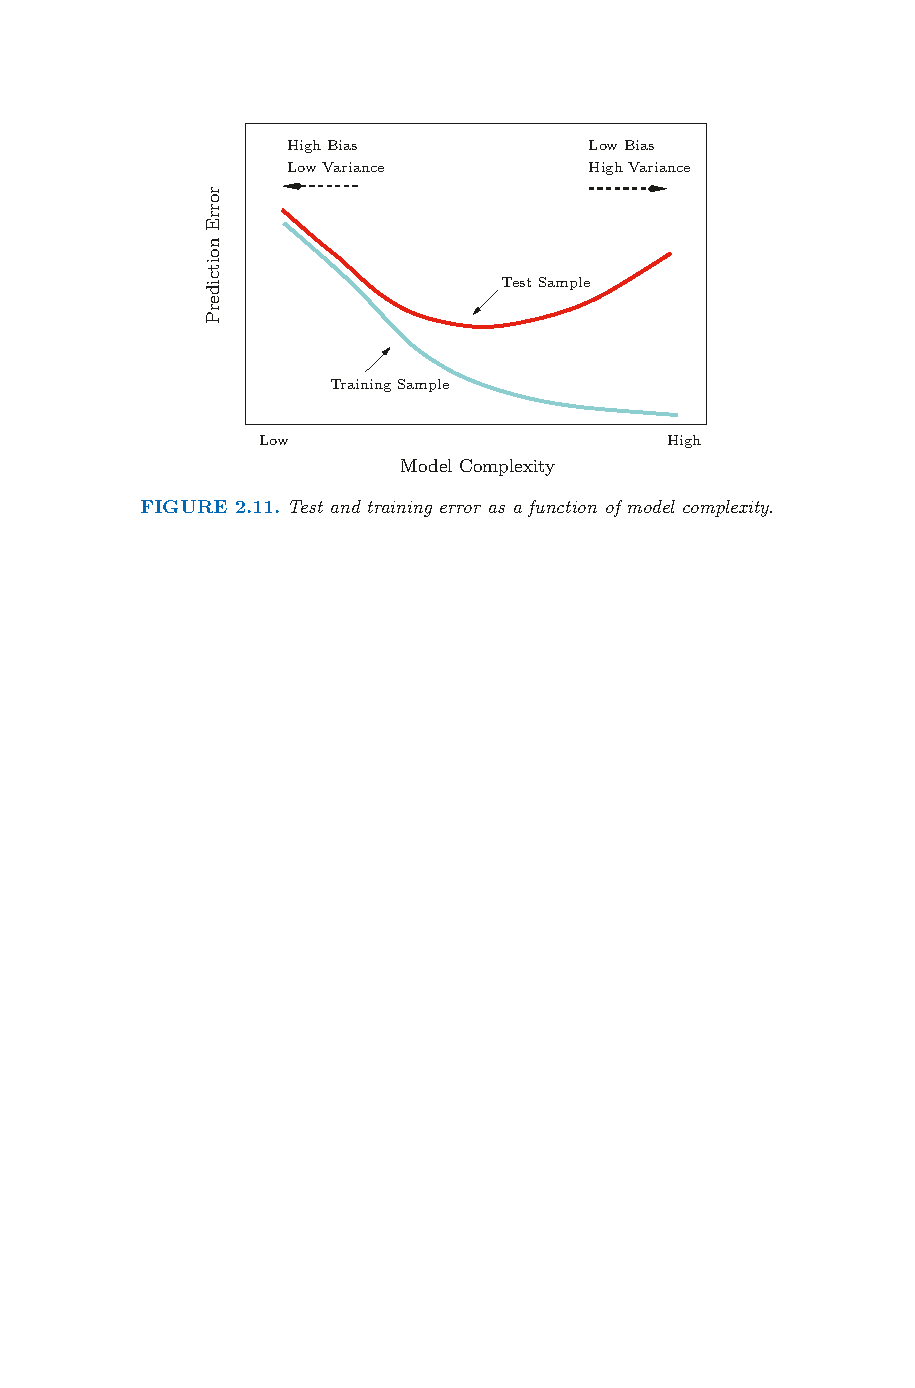
\includegraphics[width=\linewidth]{ESL-2-11.pdf}
\end{center}
\end{frame}


\begin{frame}
\frametitle{Linear vs. KNN Regressions}
\begin{itemize}
  \item Bias: How expected $\hat{f}$ is close to $f$ \hfill $f(x)-E[\hat{f}(x)]$)
  \item Variance: How variable is $\hat{f}$ itself \hfill $E[(\hat{f}(x)-E[\hat{f}(x)])^2]$
  \item Linear Regression: If $f(X)=X\beta$, then $E[\hat{\beta}]=\beta$, and
  \[MSE(\hat{f}(x))=0+(x^{T}(X^{T}X)^{-1}x)\sigma^2\]
  \vspace{-8mm}
  \begin{itemize}
    \item If $f$ is linear, then unbiased; if not, possibly (high) bias
  \end{itemize}
  \item k-Nearest Neighbors:
  \[MSE(\hat{f}(x))=\left(f(x)-{1\over k}\sum_{x_i\in N_k(x)}f(x_i)\right)^2+{\sigma^2 \over k}\]
   \vspace{-5mm}
  \begin{itemize}
    \item More flexible, can lower bias, but also increase variability
  \end{itemize}
\end{itemize}
\end{frame}


\begin{frame}
\begin{center}
  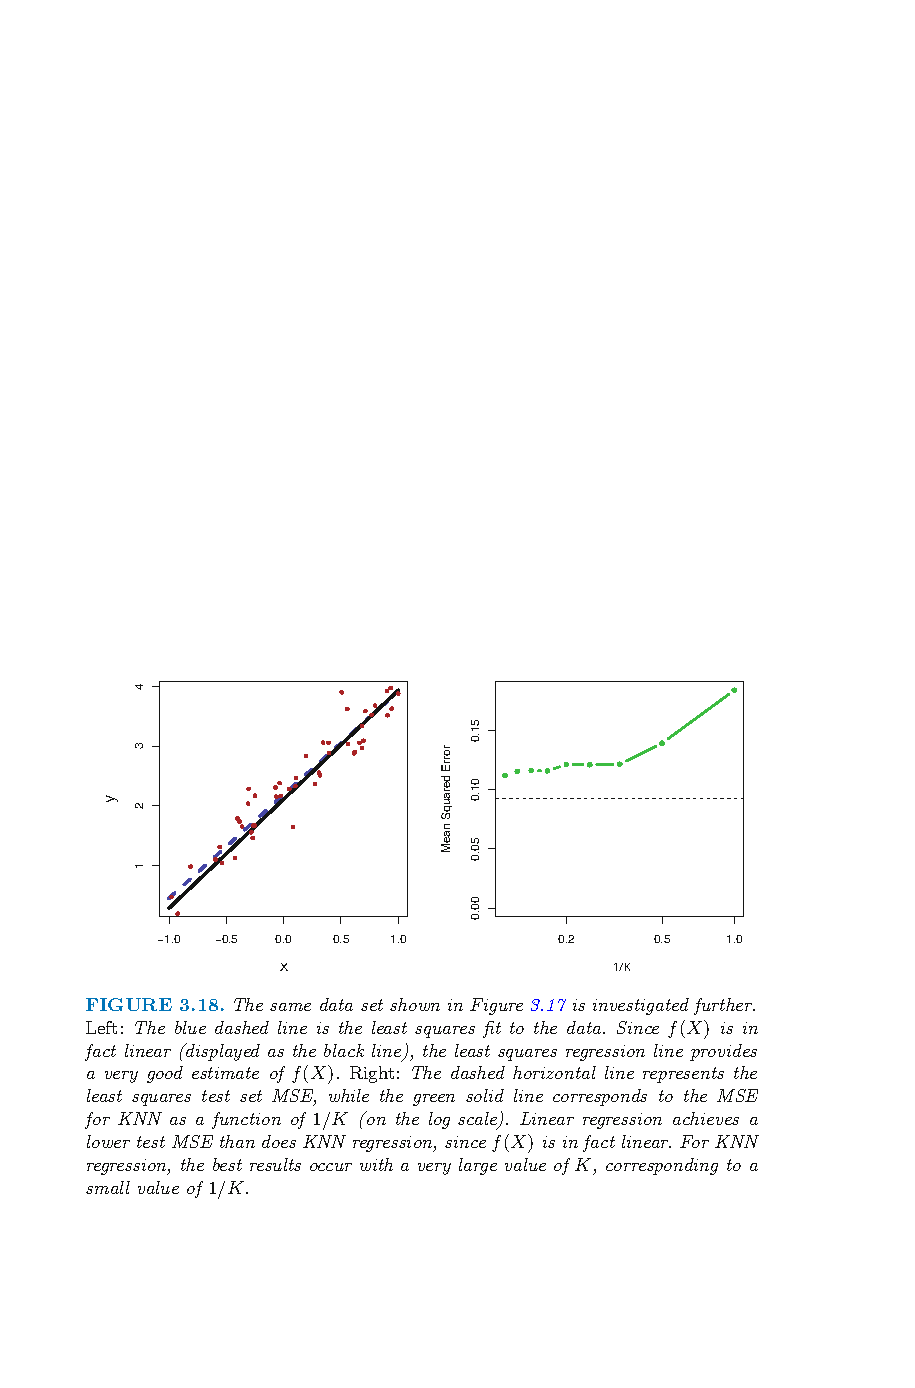
\includegraphics[width=.8\linewidth]{ISL-3-18.pdf}
\end{center}
\end{frame}


\begin{frame}
\begin{center}
  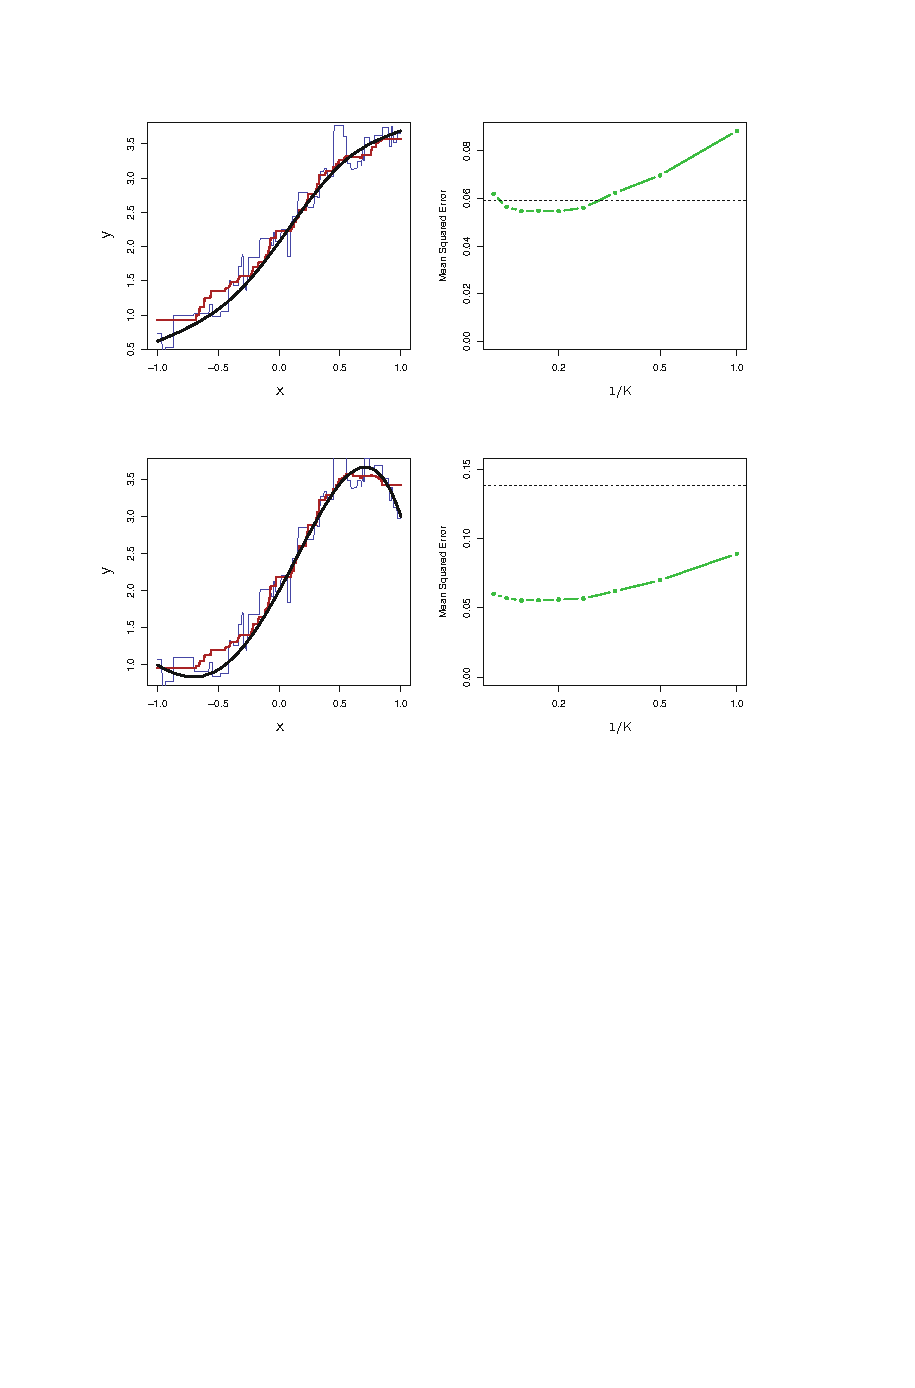
\includegraphics[width=.8\linewidth]{ISL-3-19.pdf}
\end{center}
\end{frame}


\begin{frame}
\begin{center}
  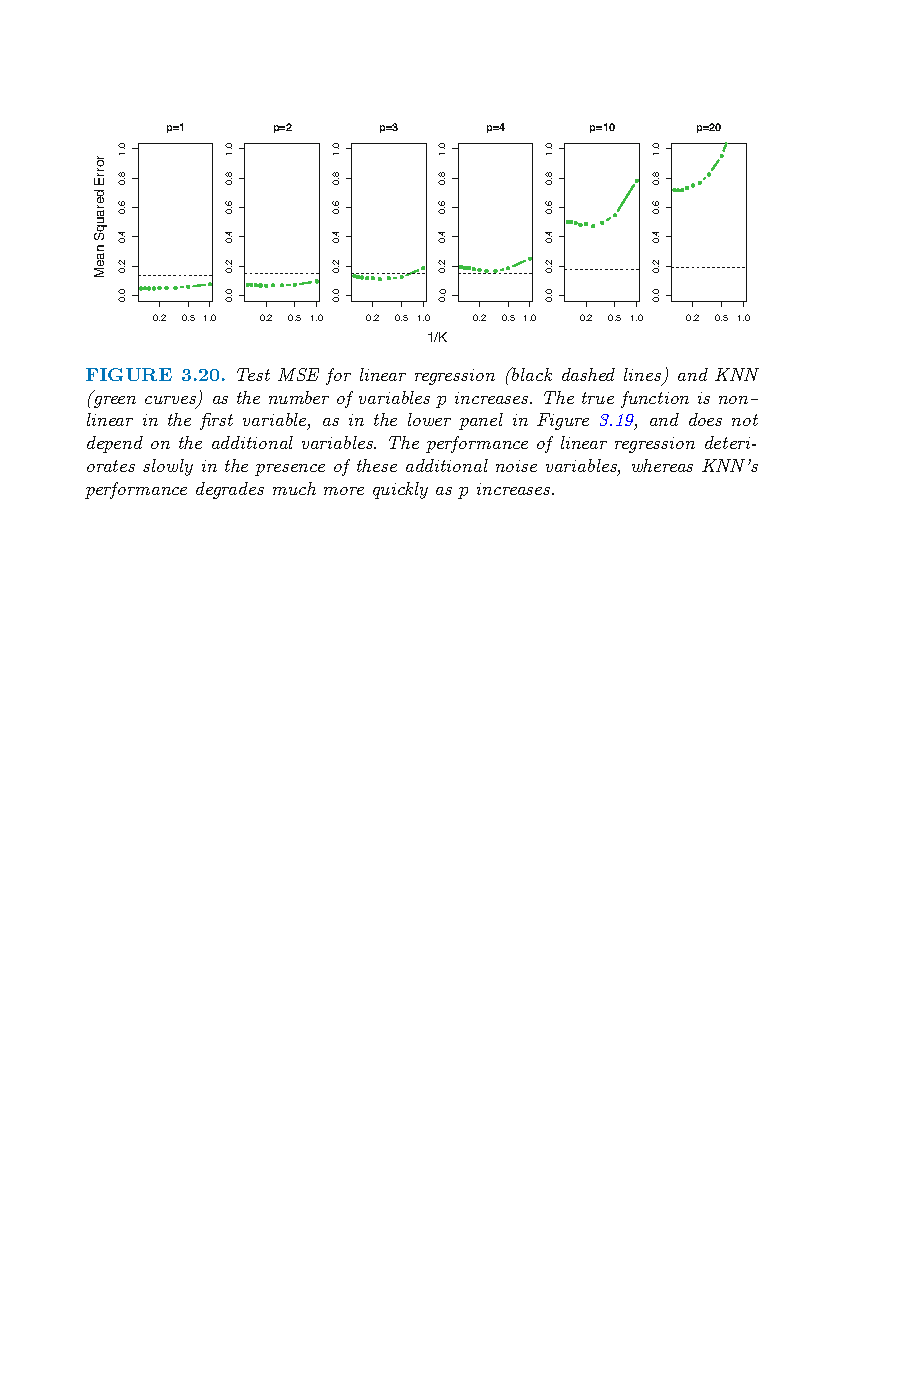
\includegraphics[width=.9\linewidth]{ISL-3-20.pdf}
\end{center}
\end{frame}


\begin{frame}
\frametitle{Curse of Dimensionality}
\begin{itemize}
  \item When $p$ increases, the model is more flexible, but there is fewer neighbors can be used
  \begin{itemize}
  \item $N$ points uniformly distributed on $[0,1]$, average distance is $1/N$
  \item $N$ points uniformly distributed on $[0,1]^2$, average distance is $1/\sqrt{N}$
  \item To achieve the same sparsity, we need $N^2$ points
  \end{itemize}
  \item Hence, as $p$ increases linearly, $N$ needs to grow exponentially in order to maintain the same sparsity
  \item Conversely, to cover the same volume, the radius needed has to increase much more faster than the dimension
\end{itemize}
\end{frame}


\begin{frame}
\begin{center}
  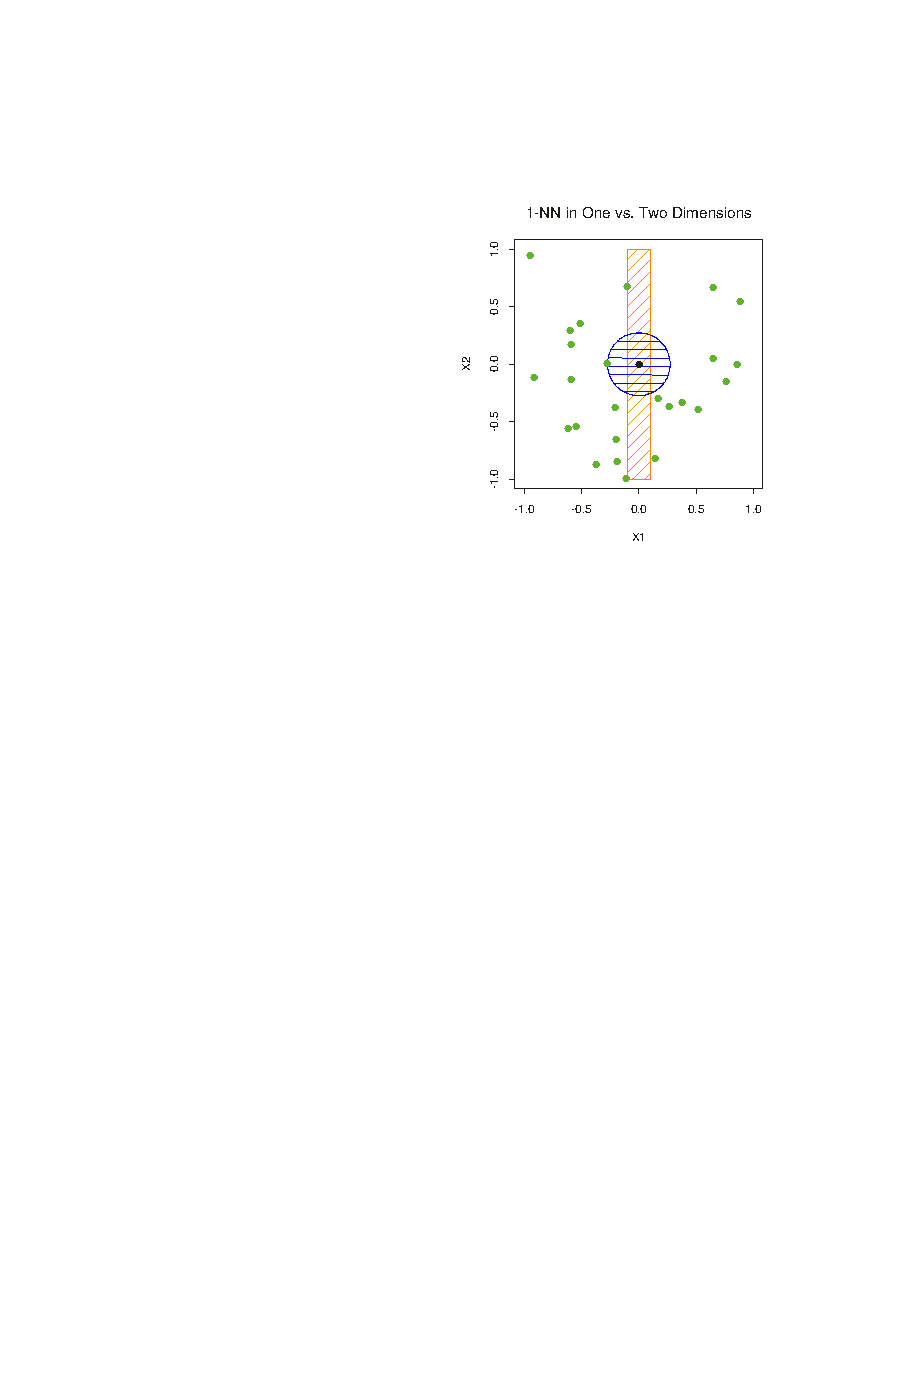
\includegraphics[width=.65\linewidth]{ESL-2-7.pdf}
\end{center}
\end{frame}


\begin{frame}
\begin{center}
  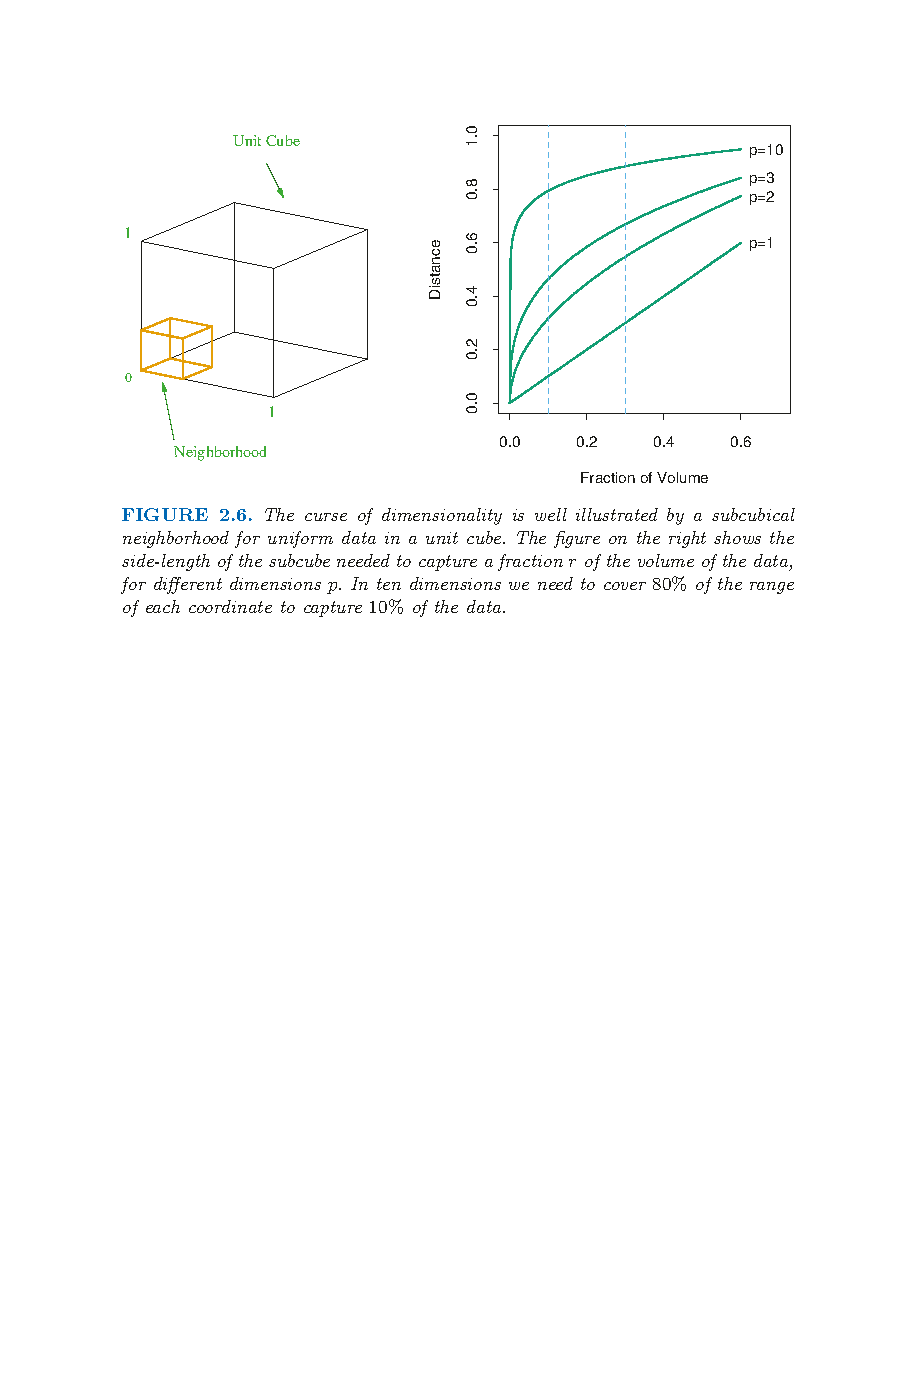
\includegraphics[width=.9\linewidth]{ESL-2-6.pdf}
\end{center}
\end{frame}


\begin{frame}
\frametitle{Classes of Restricted Estimators}
\begin{itemize}
  \item Non-parametric approach is conceptually similar to estimating infinite dimensions of parameters
  \item To overcome the curse of dimensionality, we need to restrict to some classes of $\hat{f}(x)$
  \begin{itemize}
    \item Regression with Penalty: Penalize points that are too far
    \item Kernal or Local Regression: Adding weights to closer points
    \item Basis Expansion: Do parametric estimation locally
  \end{itemize}
  \item In these cases, we need to determine the smoothing or complexity parameters, such as 
  \begin{itemize}
    \item The penalty term
    \item Width of kernel or bands
    \item The number of bases
  \end{itemize}
\end{itemize}
\end{frame}


\end{document}